\documentclass[11pt,a4paper,oneside]{report}

\usepackage[a4paper,top=22mm,bottom=22mm,left=24mm,right=24mm,headheight=15pt]{geometry}
\usepackage{fontspec}
\defaultfontfeatures{}
\setmainfont{Times New Roman}[Ligatures=TeX]
\setsansfont{Arial}[Ligatures=TeX]
\setmonofont{Consolas}[Ligatures=NoCommon]
\usepackage{microtype}
\usepackage{setspace}
\setstretch{1.08}
\usepackage{parskip}
\setlength{\parindent}{0pt}
\setlength{\emergencystretch}{2em}
\usepackage{enumitem}
\setlist{itemsep=3pt,topsep=5pt}
\usepackage{booktabs}
\usepackage{longtable}
\usepackage{tabularx}
\usepackage{array}
\usepackage{multirow}
\usepackage{amsmath}
\usepackage{amssymb}
\usepackage{graphicx}
\usepackage{xcolor}
\usepackage{listings}
\usepackage{tikz}
\usetikzlibrary{arrows.meta,positioning,shapes.geometric,fit,backgrounds,calc}
\usepackage{fancyhdr}
\usepackage{hyperref}
\usepackage{bookmark}

\definecolor{WazuhBlue}{HTML}{005EB8}
\definecolor{WazuhDark}{HTML}{17324D}
\definecolor{AlarmRed}{HTML}{B42318}
\definecolor{AlarmOrange}{HTML}{E07A17}
\definecolor{AlarmGreen}{HTML}{16794D}
\definecolor{SoftBlue}{HTML}{EAF3FB}
\definecolor{SoftGray}{HTML}{F3F5F7}
\definecolor{LineGray}{HTML}{687482}
\definecolor{CodeBg}{HTML}{F7F8FA}

\hypersetup{
  colorlinks=true,
  linkcolor=WazuhBlue,
  urlcolor=WazuhBlue,
  citecolor=WazuhDark,
  pdftitle={Logika Agregasi SIEM Alarm untuk Wazuh 4.14.7 AIO},
  pdfauthor={Dokumentasi Proyek SIEM Alarm},
  pdfsubject={Arsitektur, agregasi, risk scoring, dan operasi siem-alarm-*},
  pdfkeywords={Wazuh, SIEM, aggregation, risk scoring, OpenSearch}
}

\pagestyle{fancy}
\fancyhf{}
\fancyhead[L]{\sffamily\small SIEM Alarm Aggregation}
\fancyhead[R]{\sffamily\small Wazuh 4.14.7 AIO}
\fancyfoot[C]{\sffamily\small \thepage}
\renewcommand{\headrulewidth}{0.4pt}

\lstdefinestyle{jsonstyle}{
  basicstyle=\ttfamily\footnotesize,
  backgroundcolor=\color{CodeBg},
  frame=single,
  rulecolor=\color{LineGray!45},
  breaklines=true,
  breakatwhitespace=false,
  columns=fullflexible,
  keepspaces=true,
  showstringspaces=false,
  xleftmargin=5pt,
  xrightmargin=5pt,
  aboveskip=8pt,
  belowskip=8pt
}
\lstset{style=jsonstyle}

\DeclareRobustCommand{\code}[1]{\nolinkurl{#1}}
\newcommand{\good}[1]{\textcolor{AlarmGreen}{\textbf{#1}}}
\newcommand{\warn}[1]{\textcolor{AlarmOrange}{\textbf{#1}}}
\newcommand{\risk}[1]{\textcolor{AlarmRed}{\textbf{#1}}}
\newcommand{\projectfile}[1]{\texttt{#1}}

\newenvironment{keypoint}
  {\begin{center}\begin{minipage}{0.92\textwidth}\color{WazuhDark}\hrule\vspace{7pt}\textbf{Pokok penting.} }
  {\vspace{7pt}\hrule\end{minipage}\end{center}}

\renewcommand{\chaptername}{Bab}
\renewcommand{\contentsname}{Daftar Isi}
\renewcommand{\listfigurename}{Daftar Gambar}
\renewcommand{\listtablename}{Daftar Tabel}
\renewcommand{\figurename}{Gambar}
\renewcommand{\tablename}{Tabel}
\renewcommand{\appendixname}{Lampiran}
\renewcommand{\bibname}{Referensi}

\tikzset{
  component/.style={draw=WazuhBlue,fill=SoftBlue,rounded corners=3pt,thick,
    align=center,minimum height=12mm,text width=35mm,font=\sffamily\small},
  store/.style={draw=AlarmOrange,fill=AlarmOrange!10,rounded corners=3pt,thick,
    align=center,minimum height=12mm,text width=37mm,font=\sffamily\small},
  process/.style={draw=WazuhDark,fill=SoftGray,rounded corners=3pt,thick,
    align=center,minimum height=11mm,text width=43mm,font=\sffamily\small},
  decision/.style={diamond,draw=AlarmOrange,fill=AlarmOrange!10,thick,
    align=center,aspect=2.2,text width=27mm,font=\sffamily\scriptsize},
  endpoint/.style={draw=LineGray,fill=white,rounded corners=3pt,
    align=center,minimum height=10mm,text width=30mm,font=\sffamily\small},
  flow/.style={-{Stealth[length=2.4mm]},thick,draw=LineGray},
  dataflow/.style={-{Stealth[length=2.4mm]},thick,draw=WazuhBlue},
  writeflow/.style={-{Stealth[length=2.4mm]},thick,draw=AlarmRed},
  note/.style={draw=LineGray!60,fill=white,rounded corners=2pt,
    align=left,text width=42mm,font=\sffamily\scriptsize}
}

\begin{document}

\begin{titlepage}
  \centering
  \vspace*{15mm}
  {\sffamily\bfseries\color{WazuhBlue}\fontsize{30}{36}\selectfont
    LOGIKA AGREGASI SIEM ALARM\par}
  \vspace{5mm}
  {\sffamily\Large untuk Wazuh 4.14.7 All-in-One\par}
  \vspace{12mm}
  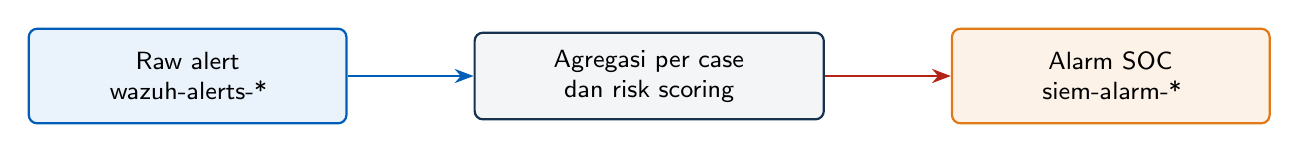
\begin{tikzpicture}
    \node[component,text width=38mm] (raw) {Raw alert\\\code{wazuh-alerts-*}};
    \node[process,right=16mm of raw,text width=42mm] (agg) {Agregasi per case\\dan risk scoring};
    \node[store,right=16mm of agg,text width=38mm] (alarm) {Alarm SOC\\\code{siem-alarm-*}};
    \draw[dataflow] (raw) -- (agg);
    \draw[writeflow] (agg) -- (alarm);
  \end{tikzpicture}
  \vfill
  {\sffamily\large Arsitektur, alur data, rumus, contoh log, reliabilitas,\par
  keamanan, operasi, dan batas penggunaan nyata\par}
  \vfill
  \begin{tabular}{rl}
    Baseline: & Wazuh 4.14.7 AIO / single node\\
    Bucket: & 60 menit, UTC\\
    Jadwal: & setiap 5 menit\\
    Dokumen keluaran: & \code{alarm_state} dan \code{alarm_escalation}\\
    Tanggal dokumen: & 26 Agustus 2026\\
  \end{tabular}
  \vspace{15mm}

  {\small Dokumen ini menjelaskan perilaku implementasi pada
  \projectfile{siem\_alarm\_scoring\_final.py}. Ia bukan pengganti hasil
  load test dan validasi pada server produksi tertentu.}
\end{titlepage}

\pagenumbering{roman}
\tableofcontents
\clearpage
\listoffigures
\clearpage
\listoftables
\clearpage
\pagenumbering{arabic}

\chapter{Ringkasan Eksekutif}

Sistem agregasi SIEM Alarm dibuat untuk mengurangi jumlah alert mentah yang harus
dibaca analis tanpa menghapus bukti asalnya. Wazuh tetap menjadi mesin deteksi.
Setiap dokumen Wazuh yang cocok tetap disimpan pada \code{wazuh-alerts-*}; sistem
tambahan ini membaca dokumen tersebut, menyatukan alert yang dianggap satu kasus,
memberikan skor risiko, lalu menulis ringkasannya ke \code{siem-alarm-*}.

Definisi default satu kasus adalah kombinasi \code{agent.id}, \code{rule.id}, dan
bucket waktu satu jam dalam UTC. Source IP, destination IP, port, user, URL, dan
file tidak hilang. Pada mode default semuanya menjadi evidence di dalam satu alarm,
bukan pemecah alarm. Karena itu serangan dari botnet atau rotating source IP tidak
serta-merta menghasilkan ratusan kartu alarm terpisah.

Sistem menghasilkan dua tipe dokumen. \code{alarm_state} adalah keadaan terbaru
dari satu kasus dan ditulis ulang menggunakan document ID yang sama.
\code{alarm_escalation} adalah catatan immutable ketika risiko pertama kali masuk
level yang dipantau atau naik ke level lebih tinggi. Pemisahan ini membuat dashboard
dapat menampilkan keadaan terakhir, sementara aplikasi eksternal dapat mengonsumsi
stream perubahan risiko.

\begin{keypoint}
Status teknis paket adalah siap untuk staging atau shadow run pada baseline yang
ditentukan. Status produksi baru dapat diberikan setelah field audit, validasi TLS
dan role, rekonsiliasi count dengan raw alert, pengukuran lag, serta load test pada
host Wazuh yang sebenarnya selesai.
\end{keypoint}

\chapter{Tujuan dan Lingkup Desain}

Tujuan utama sistem bukan mengganti korelasi Wazuh, melainkan membentuk lapisan
prioritisasi operasional untuk SOC. Wazuh menentukan bahwa sebuah event adalah
alert melalui decoder dan rule. Engine agregasi baru bekerja setelah keputusan
tersebut dibuat.

Baseline yang menjadi sasaran adalah:

\begin{itemize}
  \item Ubuntu dengan instalasi Wazuh all-in-one;
  \item Wazuh Manager, Wazuh Indexer, dan Wazuh Dashboard versi 4.14.7;
  \item Filebeat OSS 7.10.2;
  \item satu node Indexer, sehingga template memakai satu primary shard dan nol replica;
  \item sekitar 5 sampai 25 agent, dengan kapasitas aktual ditentukan EPS dan cardinality;
  \item eksekusi serial setiap lima menit melalui systemd timer;
  \item bucket tetap 60 menit.
\end{itemize}

Yang tidak otomatis tercakup adalah deployment distributed, multi-node Indexer,
container, Wazuh Cloud, source index dengan pembagian tanggal non-UTC, serta
workflow incident management seperti acknowledge, assignment, atau resolved.
Field \code{alarm.status} hanya menyatakan lifecycle bucket: \code{open} atau
\code{finalized}.

Sistem juga bukan UEBA, bukan machine learning, dan bukan pengganti penilaian
risiko organisasi. Skor yang dihasilkan adalah heuristik deterministik agar prioritas
dapat dijelaskan dan diaudit.

\chapter{Komponen dan Berkas Proyek}

Implementasi dibagi menjadi berkas yang memiliki tanggung jawab jelas.

\begin{longtable}{>{\ttfamily\raggedright\arraybackslash}p{0.42\textwidth}p{0.50\textwidth}}
\toprule
\normalfont\textbf{Berkas} & \textbf{Fungsi}\\
\midrule
\endhead
siem\_alarm\_scoring\_final.py & Engine query, agregasi, scoring, checkpoint, \code{\_mget}, dan two-phase \code{\_bulk}.\\
wazuh\_field\_audit\_final.py & Mengambil sampel raw alert dan melaporkan field yang benar-benar ada.\\
config.siem\_alarm.example.json & Baseline konfigurasi runtime dan seluruh guardrail.\\
assets.example.json & Contoh schema nilai aset; bukan inventory production.\\
siem\_alarm\_template\_final.json & Mapping dan setting untuk index hasil.\\
siem\_alarm\_ism\_policy.json & Retensi default 90 hari untuk index hasil baru.\\
setup\_siem\_alarm\_final.sh & Preflight, backup, instalasi, user Linux, systemd, dan logrotate.\\
tests/ & Regression test untuk fungsi inti, retry, idempotensi, cap, dan checkpoint.\\
\bottomrule
\end{longtable}

Konfigurasi dan inventory aset dipasang root-owned tetapi dapat dibaca group service.
Secret tidak disimpan di JSON; password dibaca dari environment file systemd.
Mutable checkpoint dipisahkan ke \code{/var/lib/wazuh-risk-scoring}, sedangkan log
ditulis ke direktori aplikasi yang secara eksplisit diizinkan oleh sandbox systemd.

\chapter{Topologi Wazuh All-in-One dengan Agregasi}

Gambar berikut menunjukkan komponen logis pada satu host AIO. Panah biru adalah
alur raw alert atau read, sedangkan panah merah adalah penulisan dokumen hasil.

\begin{figure}[ht]
\centering
\resizebox{0.98\textwidth}{!}{%
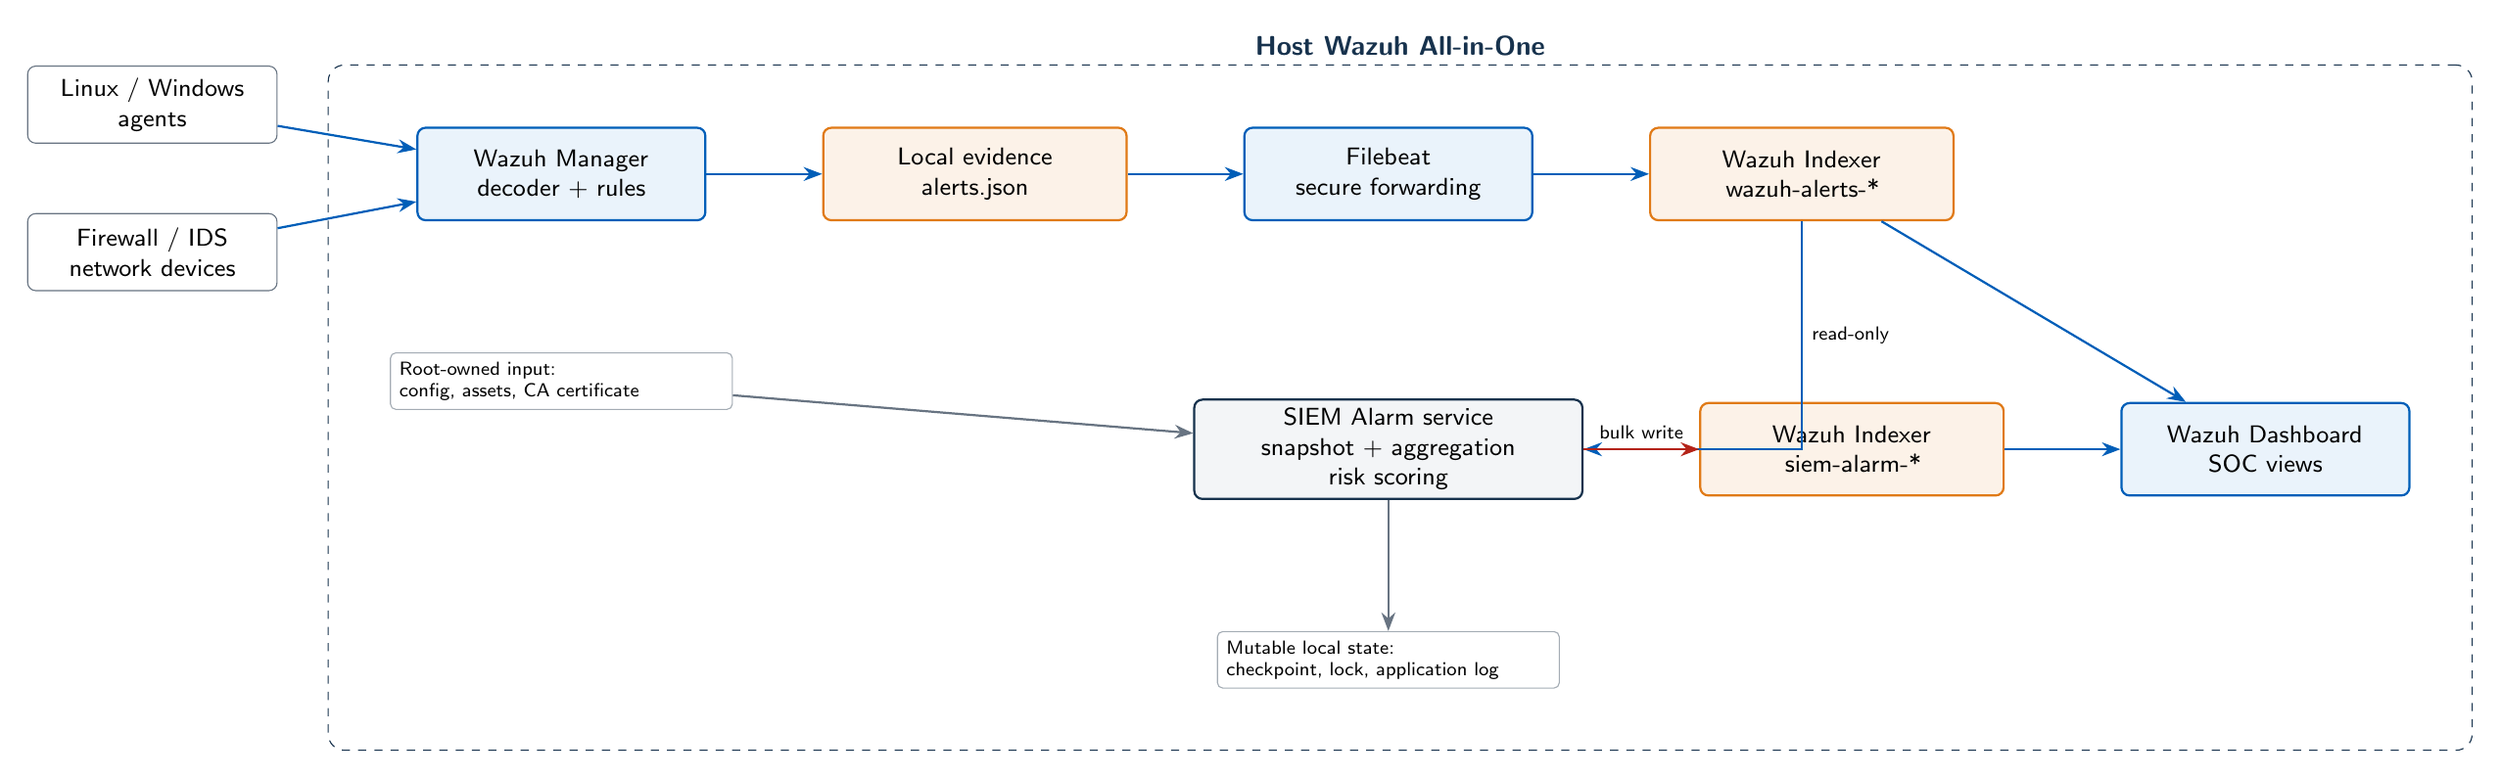
\begin{tikzpicture}[node distance=11mm and 13mm]
  \node[endpoint] (linux) {Linux / Windows\\agents};
  \node[endpoint,below=9mm of linux] (network) {Firewall / IDS\\network devices};

  \node[component,right=18mm of linux,yshift=-9mm] (manager) {Wazuh Manager\\decoder + rules};
  \node[store,right=15mm of manager] (alertsjson) {Local evidence\\\code{alerts.json}};
  \node[component,right=15mm of alertsjson] (filebeat) {Filebeat\\secure forwarding};
  \node[store,right=15mm of filebeat] (rawindex) {Wazuh Indexer\\\code{wazuh-alerts-*}};

  \node[process,below=23mm of filebeat,text width=48mm] (scorer) {SIEM Alarm service\\snapshot + aggregation\\risk scoring};
  \node[store,right=15mm of scorer] (alarmindex) {Wazuh Indexer\\\code{siem-alarm-*}};
  \node[component,right=15mm of alarmindex] (dashboard) {Wazuh Dashboard\\SOC views};

  \node[note,below=17mm of manager] (config) {Root-owned input:\\config, assets, CA certificate};
  \node[note,below=17mm of scorer] (state) {Mutable local state:\\checkpoint, lock, application log};

  \draw[dataflow] (linux) -- (manager);
  \draw[dataflow] (network) -- (manager);
  \draw[dataflow] (manager) -- (alertsjson);
  \draw[dataflow] (alertsjson) -- (filebeat);
  \draw[dataflow] (filebeat) -- (rawindex);
  \draw[dataflow] (rawindex) |- node[pos=.25,right,font=\scriptsize\sffamily]{read-only} (scorer);
  \draw[writeflow] (scorer) -- node[above,font=\scriptsize\sffamily]{bulk write} (alarmindex);
  \draw[dataflow] (rawindex) -- (dashboard);
  \draw[dataflow] (alarmindex) -- (dashboard);
  \draw[flow] (config) -- (scorer);
  \draw[flow] (scorer) -- (state);

  \begin{scope}[on background layer]
    \node[draw=WazuhDark,dashed,rounded corners=6pt,fit=(manager)(alertsjson)(filebeat)(rawindex)(scorer)(alarmindex)(dashboard)(config)(state),inner sep=8mm,
      label={[font=\sffamily\bfseries\color{WazuhDark}]above:Host Wazuh All-in-One}] {};
  \end{scope}
\end{tikzpicture}%
}
\caption{Topologi logis Wazuh AIO setelah sistem agregasi diterapkan.}
\end{figure}

Raw index dan alarm index dapat berada pada cluster Indexer yang sama, tetapi hak
aksesnya berbeda. Runtime hanya membaca \code{wazuh-alerts-*}; ia tidak mengubah
atau menghapus bukti asal. Pada \code{siem-alarm-*}, runtime memerlukan read untuk
membaca state sebelumnya, index/create untuk menulis, dan create-index agar index
harian pertama dapat dibuat setelah template terpasang.

\chapter{Flowchart Proses Satu Run}

Satu run kalender bersifat bounded dan fail-closed. Kegagalan validasi, shard,
scroll, bulk, atau cap menghentikan run dan mencegah checkpoint maju.

Flowchart pada halaman berikut dapat dibaca sebagai lima fase berurutan:

\begin{enumerate}
  \item \textbf{preflight runtime}: lock, konfigurasi, TLS, secret, dan inventory;
  \item \textbf{window planning}: memilih current bucket dan closed bucket yang eligible;
  \item \textbf{snapshot acquisition}: membaca exact daily index sampai seluruh hit lengkap;
  \item \textbf{materialization}: membentuk case, scoring, event escalation, dan state;
  \item \textbf{commit recovery}: checkpoint hanya maju bila semua window sukses.
\end{enumerate}

Cabang menuju \emph{Fail run} bukan sekadar error handling. Cabang tersebut adalah
kontrol integritas untuk memastikan dashboard tidak menerima snapshot yang diketahui
tidak lengkap. Raw alert tetap tersedia, sehingga run dapat diulang setelah penyebab
masalah diselesaikan.

\begin{figure}[ht]
\centering
\resizebox{0.96\textwidth}{!}{%
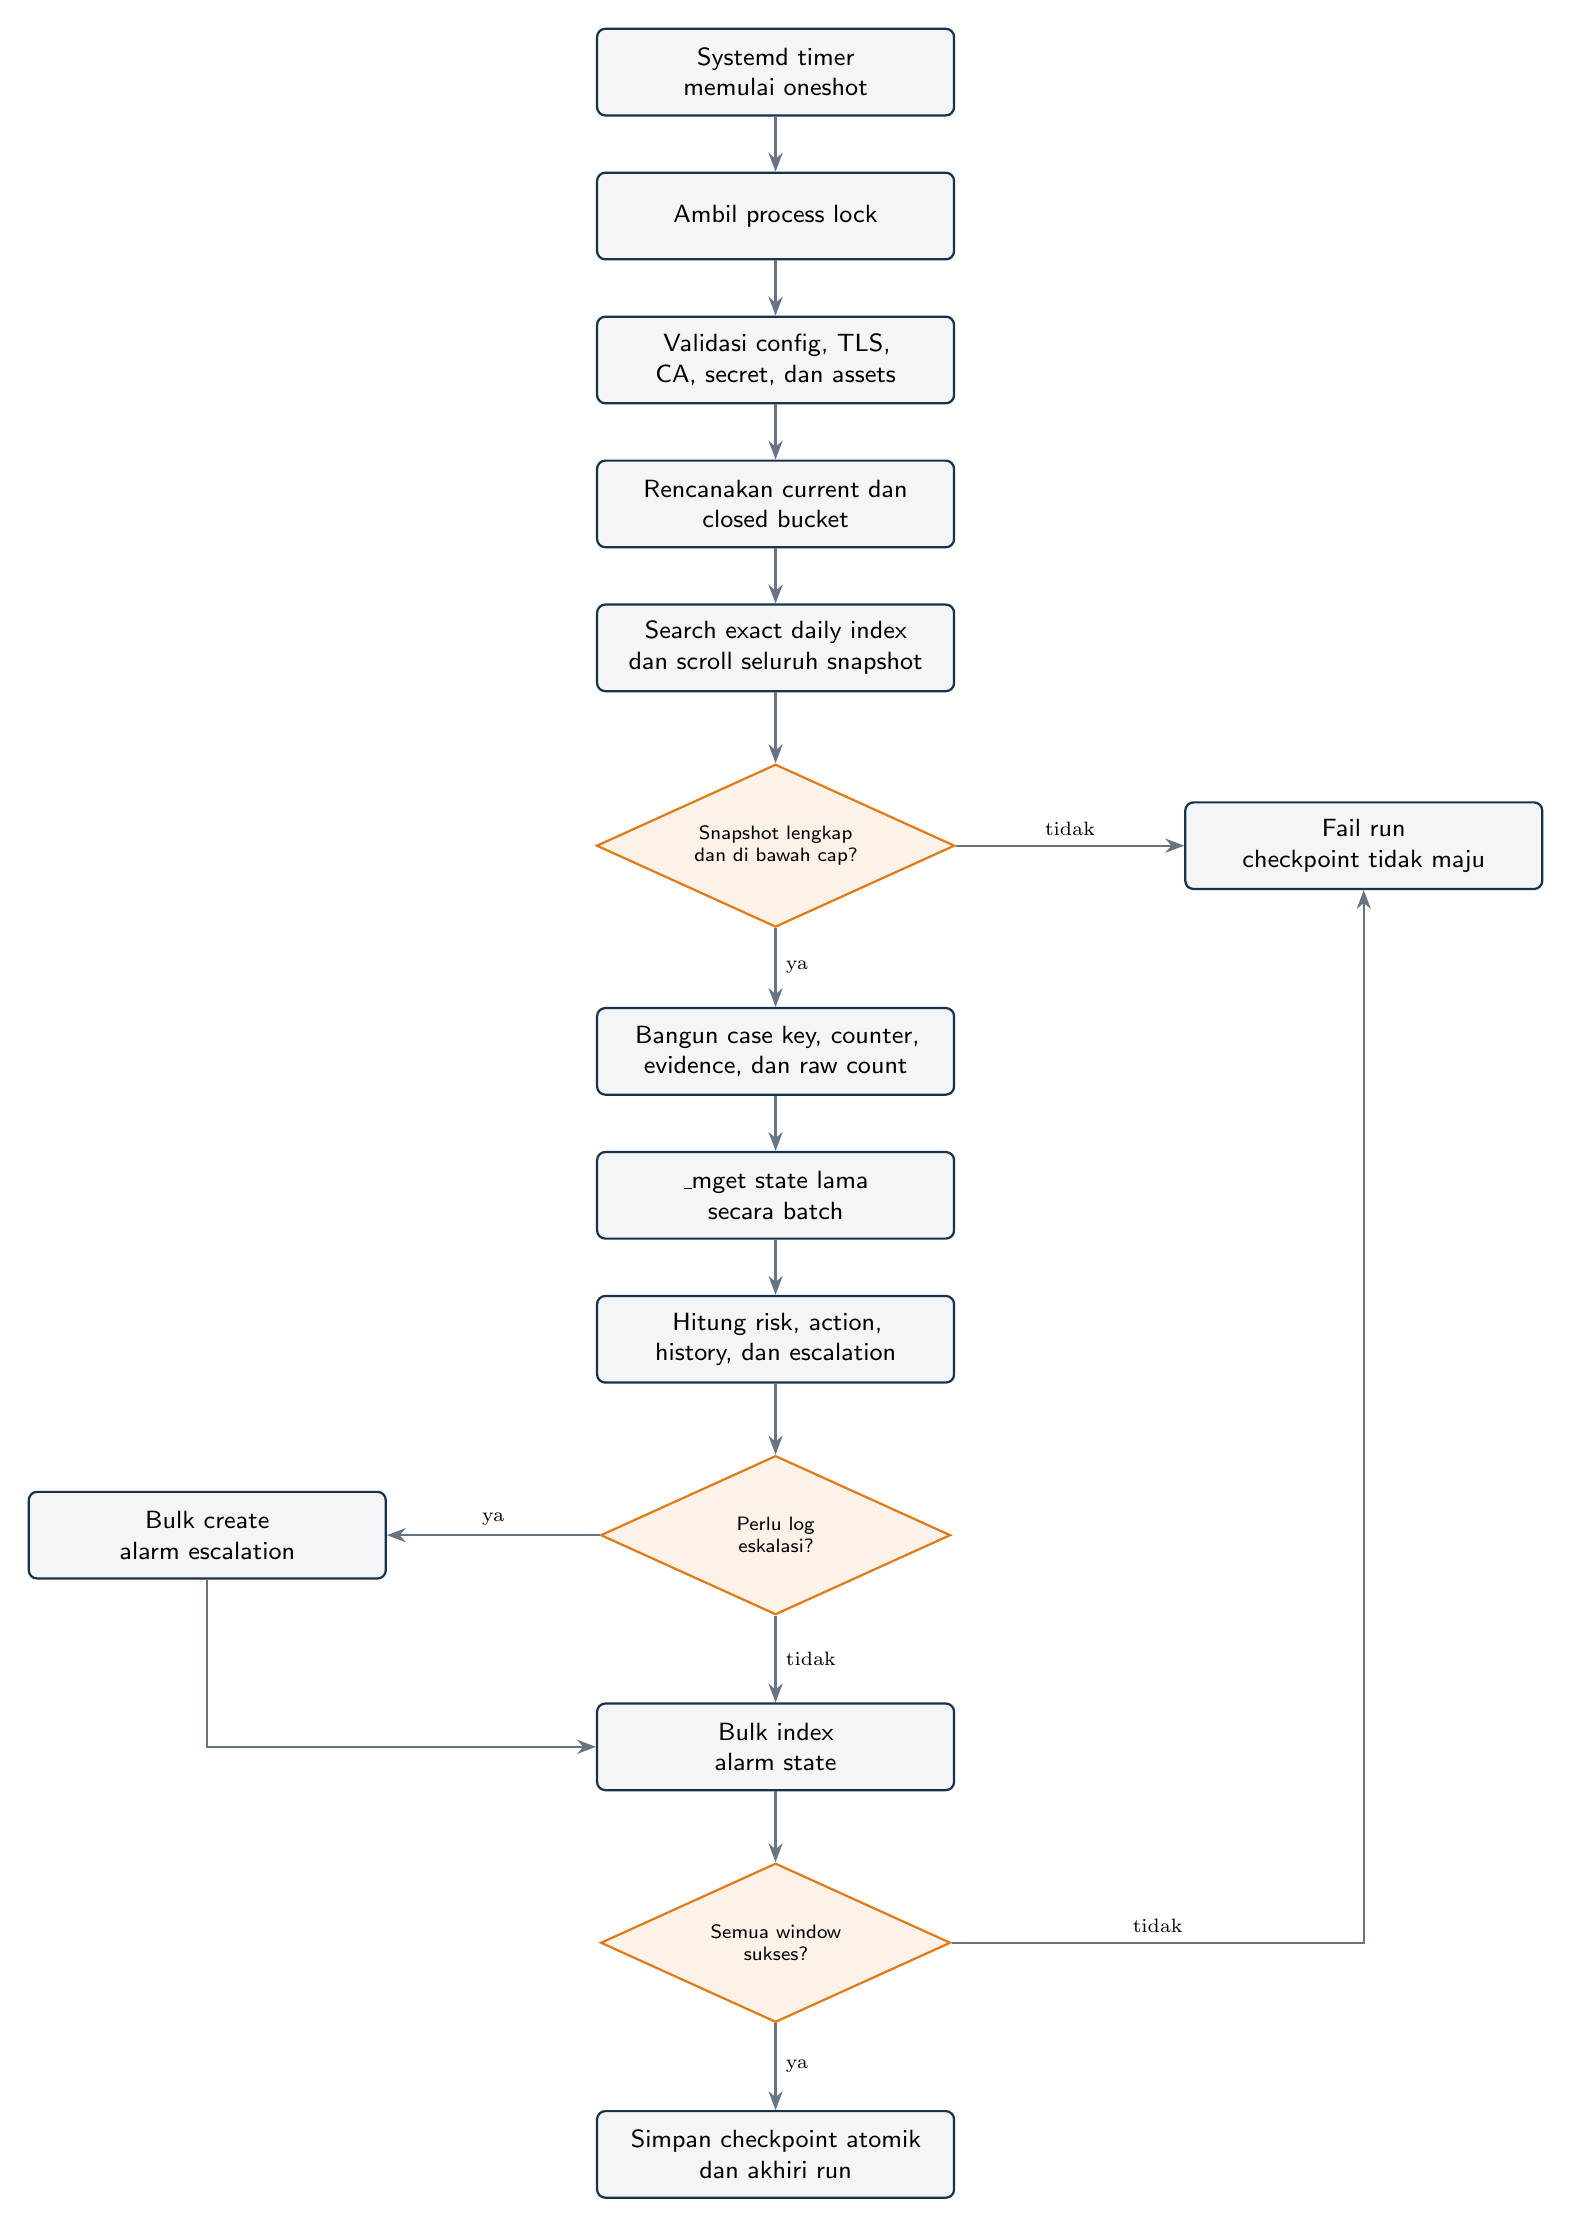
\begin{tikzpicture}[node distance=7mm and 16mm]
  \node[process] (timer) {Systemd timer\\memulai oneshot};
  \node[process,below=of timer] (lock) {Ambil process lock};
  \node[process,below=of lock] (load) {Validasi config, TLS,\\CA, secret, dan assets};
  \node[process,below=of load] (plan) {Rencanakan current dan\\closed bucket};
  \node[process,below=of plan] (search) {Search exact daily index\\dan scroll seluruh snapshot};
  \node[decision,below=9mm of search] (valid) {Snapshot lengkap\\dan di bawah cap?};

  \node[process,right=29mm of valid] (abort) {Fail run\\checkpoint tidak maju};
  \node[process,below=10mm of valid] (aggregate) {Bangun case key, counter,\\evidence, dan raw count};
  \node[process,below=of aggregate] (mget) {\code{\_mget} state lama\\secara batch};
  \node[process,below=of mget] (score) {Hitung risk, action,\\history, dan escalation};
  \node[decision,below=9mm of score] (escalate) {Perlu log\\eskalasi?};
  \node[process,left=27mm of escalate] (event) {Bulk \code{create}\\alarm escalation};
  \node[process,below=11mm of escalate] (statewrite) {Bulk \code{index}\\alarm state};
  \node[decision,below=9mm of statewrite] (allok) {Semua window\\sukses?};
  \node[process,below=11mm of allok] (checkpoint) {Simpan checkpoint atomik\\dan akhiri run};

  \draw[flow] (timer) -- (lock);
  \draw[flow] (lock) -- (load);
  \draw[flow] (load) -- (plan);
  \draw[flow] (plan) -- (search);
  \draw[flow] (search) -- (valid);
  \draw[flow] (valid) -- node[above,font=\scriptsize]{tidak} (abort);
  \draw[flow] (valid) -- node[right,font=\scriptsize]{ya} (aggregate);
  \draw[flow] (aggregate) -- (mget);
  \draw[flow] (mget) -- (score);
  \draw[flow] (score) -- (escalate);
  \draw[flow] (escalate) -- node[above,font=\scriptsize]{ya} (event);
  \draw[flow] (event) |- (statewrite);
  \draw[flow] (escalate) -- node[right,font=\scriptsize]{tidak} (statewrite);
  \draw[flow] (statewrite) -- (allok);
  \draw[flow] (allok) -- node[right,font=\scriptsize]{ya} (checkpoint);
  \draw[flow] (allok.east) -| node[pos=.25,above,font=\scriptsize]{tidak} (abort.south);
\end{tikzpicture}%
}
\caption{Flowchart satu eksekusi engine agregasi.}
\end{figure}

Poin pentingnya adalah state tidak ditulis sebelum event eskalasi yang bergantung
padanya berhasil dibuat. Jika bulk escalation gagal sebagian, state terkait ditahan.
Run berikutnya aman mengulang karena event memakai create-only ID deterministik dan
state memakai index ID deterministik.

\chapter{Model Waktu dan Bucket}

Semua identitas bucket dihitung dalam UTC. Timestamp Wazuh yang memakai bentuk
\code{+0000}, \code{-0500}, atau offset lain dinormalisasi terlebih dahulu.
Untuk konfigurasi baseline 60 menit, timestamp berikut semuanya masuk bucket yang
sama:

\begin{lstlisting}
2026-04-21T02:00:00Z
2026-04-21T02:42:05.483+0000
2026-04-21T09:58:33+0700
\end{lstlisting}

Ketiganya berada pada rentang setengah terbuka:

\[
  \texttt{2026-04-21T02:00:00Z}
  \leq t <
  \texttt{2026-04-21T03:00:00Z}
\]

Current bucket dihitung ulang dari boundary sampai waktu run. Bucket tertutup baru
eligible setelah delay default tujuh menit. Dengan timer lima menit, finalisasi
normal terjadi pada tick sekitar boundary ditambah sepuluh menit, bukan tepat tujuh
menit.

\begin{figure}[ht]
\centering
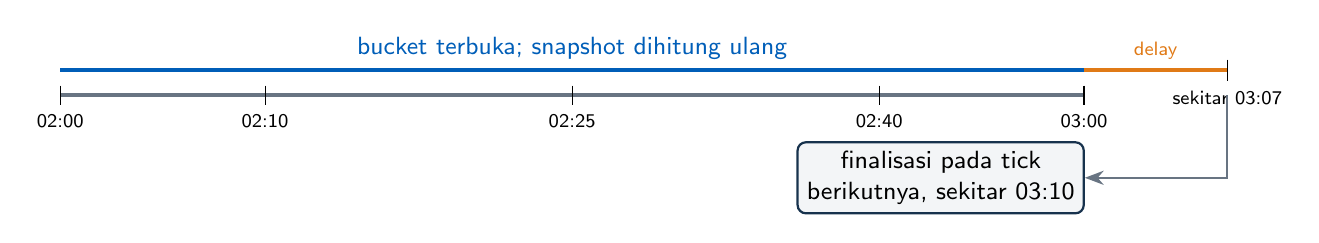
\begin{tikzpicture}[x=1.3cm,y=1cm]
  \draw[very thick,LineGray] (0,0) -- (10,0);
  \foreach \x/\lab in {0/02:00,2/02:10,5/02:25,8/02:40,10/03:00}
    \draw (\x,0.12)--(\x,-0.12) node[below,font=\scriptsize\sffamily]{\lab};
  \draw[very thick,WazuhBlue] (0,0.32) -- (10,0.32)
    node[midway,above,font=\small\sffamily]{bucket terbuka; snapshot dihitung ulang};
  \draw[very thick,AlarmOrange] (10,0.32) -- (11.4,0.32)
    node[midway,above,font=\scriptsize\sffamily]{delay};
  \draw (11.4,0.45)--(11.4,0.18) node[below,font=\scriptsize\sffamily]{sekitar 03:07};
  \node[process,text width=34mm,minimum height=8mm] (finalize) at (8.6,-1.05) {finalisasi pada tick\\berikutnya, sekitar 03:10};
  \draw[flow] (11.4,0) |- (finalize.east);
\end{tikzpicture}
\caption{Lifecycle waktu satu bucket baseline.}
\end{figure}

Alert yang baru masuk Indexer setelah bucket difinalisasi tidak direvisi otomatis.
Ia memerlukan backfill eksplisit. Karena itu delay harus lebih besar daripada lag
end-to-end normal dan p99 lag perlu dimonitor.

\chapter{Definisi ``Alert yang Sama''}

Mode default \code{coarse} menghasilkan key:

\begin{lstlisting}
coarse|<agent.id>|<rule.id>|<bucket_start_UTC>
\end{lstlisting}

Dengan demikian dua source IP, dua username, atau dua URL berbeda tetap menjadi
satu alarm ketika agent, rule, dan bucket sama. Ini cocok untuk suppression dan
pengelompokan attack wave, tetapi belum tentu cocok untuk seluruh rule.

\begin{table}[ht]
\centering
\caption{Mode deduplikasi yang tersedia.}
\begin{tabularx}{\textwidth}{>{\ttfamily}l X X}
\toprule
\normalfont\textbf{Mode} & \textbf{Field identitas} & \textbf{Penggunaan yang disarankan}\\
\midrule
coarse & agent.id, rule.id, bucket & Default; noise suppression per agent dan rule.\\
target\_aware & coarse + dstip & Sensor IDS/firewall yang mengamati banyak server tujuan.\\
target\_port\_aware & target + dstport + proto & Rule jaringan ketika layanan tujuan harus dipisahkan.\\
file\_aware & coarse + file path & FIM/malware ketika setiap path harus menjadi alarm tersendiri.\\
\bottomrule
\end{tabularx}
\end{table}

Mode dapat ditetapkan global dan dioverride per \code{rule.id}. Source IP sengaja
tidak menjadi split key pada mode yang tersedia. Jika organisasi memerlukan alarm
per source IP atau per username, implementasi perlu mode identitas tambahan dan
migrasi destination/checkpoint yang terkontrol.

Perubahan mode mengubah identitas kasus. Engine menyimpan hash identitas konfigurasi
di checkpoint dan akan fail-closed bila konfigurasi identitas berubah secara diam-diam.

\chapter{Agregasi Source IP dan Evidence}

Source IP yang berbeda tidak menggantikan satu sama lain. Engine menggunakan
counter per nilai. Misalkan terdapat 75 raw alert:

\begin{center}
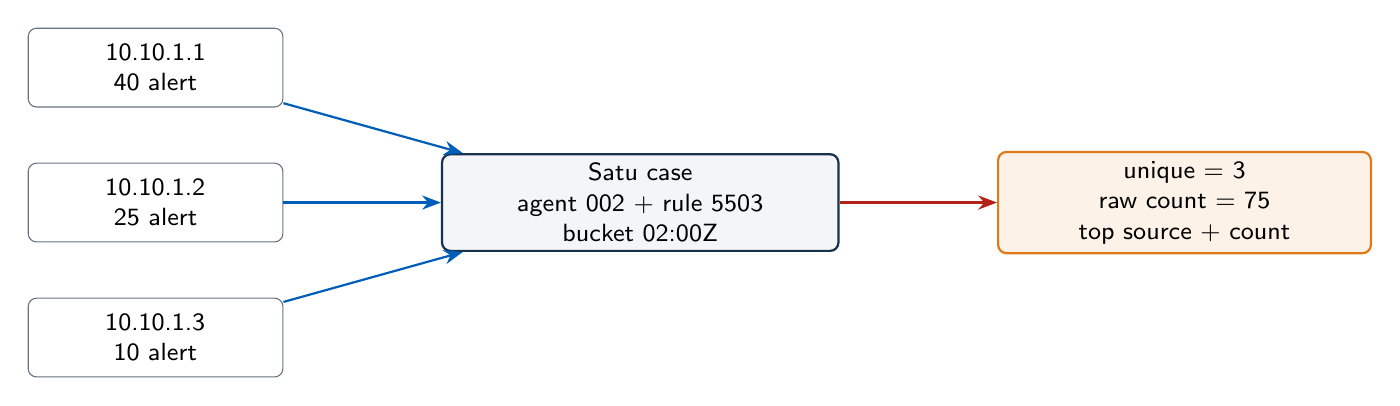
\begin{tikzpicture}[node distance=7mm and 12mm]
  \node[endpoint] (ip1) {10.10.1.1\\40 alert};
  \node[endpoint,below=of ip1] (ip2) {10.10.1.2\\25 alert};
  \node[endpoint,below=of ip2] (ip3) {10.10.1.3\\10 alert};
  \node[process,right=20mm of ip2,text width=48mm] (case) {Satu case\\agent 002 + rule 5503\\bucket 02:00Z};
  \node[store,right=20mm of case,text width=45mm] (summary) {unique = 3\\raw count = 75\\top source + count};
  \draw[dataflow] (ip1) -- (case);
  \draw[dataflow] (ip2) -- (case);
  \draw[dataflow] (ip3) -- (case);
  \draw[writeflow] (case) -- (summary);
\end{tikzpicture}
\end{center}

Hasil ringkasannya:

\begin{lstlisting}
"source_observed": {
  "srcip_unique_count": 3,
  "srcip_samples": ["10.10.1.1", "10.10.1.2", "10.10.1.3"],
  "top_srcip": [
    {"value": "10.10.1.1", "count": 40},
    {"value": "10.10.1.2", "count": 25},
    {"value": "10.10.1.3", "count": 10}
  ]
}
\end{lstlisting}

\code{srcip\_unique\_count} menghitung semua nilai unik yang dilihat snapshot.
\code{srcip\_samples} menyimpan maksimal 20 nilai dan \code{top\_srcip} maksimal
10 pasangan nilai-count secara default. Bila terdapat 100 IP unik, count tetap 100,
tetapi hanya nilai teratas yang dimaterialisasi ke alarm. Daftar diurutkan menurut
frekuensi menurun lalu teks nilai, bukan menurut waktu kedatangan.

Nilai yang tidak masuk batas sampel tidak hilang dari sistem: raw document tetap
berada pada \code{wazuh-alerts-*}. Batas tersebut hanya menjaga ukuran dokumen alarm.

\chapter{Field Extraction dan Normalisasi}

Engine mencari observed field melalui beberapa alias yang lazim ditemukan pada
Wazuh dan ECS. Contoh source IP meliputi \code{data.srcip}, \code{data.src\_ip},
\code{srcip}, \code{source.ip}, dan beberapa field Windows. Destination IP dapat
jatuh kembali ke \code{agent.ip} bila tidak ada destination eksplisit.

Observed data yang diringkas mencakup:

\begin{itemize}
  \item source IP;
  \item destination IP, port, dan protocol;
  \item URL dan user agent;
  \item username;
  \item file path dan hash;
  \item CVE dan SCA check ID.
\end{itemize}

Protocol angka umum dinormalisasi: 6 menjadi TCP, 17 menjadi UDP, dan 1 menjadi
ICMP. Nilai kosong, tanda minus, \code{0.0.0.0}, dan \code{::} diperlakukan sebagai
tidak terobservasi.

Field audit wajib dijalankan sebelum production karena decoder dan custom rule
dapat menghasilkan path berbeda. Menambahkan path ke \code{source\_includes}
hanya membuat field ikut dikirim oleh Indexer. Jika nama tersebut bukan alias yang
dikenali fungsi ekstraksi, kode alias juga harus diperluas dan diuji.

\chapter{Asset Value dan Sumber Kepercayaan}

Asset Value adalah komponen pertama skor. Urutan sumbernya:

\begin{enumerate}
  \item inventory \code{assets.json}, lookup berdasarkan \code{agent.id};
  \item lookup berdasarkan \code{agent.name} jika ID tidak ditemukan;
  \item label resmi \code{agent.labels.*} sebagai fallback;
  \item nilai default 3 atau Medium disertai warning.
\end{enumerate}

\begin{table}[ht]
\centering
\caption{Skala Asset Value.}
\begin{tabularx}{0.88\textwidth}{c l X}
\toprule
\textbf{Nilai} & \textbf{Kategori} & \textbf{Contoh}\\
\midrule
5 & Critical & Database inti, AD/LDAP, sistem keselamatan, firewall kritikal.\\
4 & High & Web server produksi, mail, VPN, sensor IDS penting.\\
3 & Medium & Application server internal atau aset tanpa klasifikasi khusus.\\
2 & Low & Workstation biasa, printer, endpoint berdampak rendah.\\
1 & Minimal & Development/test yang terisolasi.\\
\bottomrule
\end{tabularx}
\end{table}

Inventory divalidasi secara ketat. Nilai harus integer 1 sampai 5, category harus
sesuai, field tidak dikenal ditolak, dan mismatch nama untuk agent ID yang sama
menghentikan run. Pemeriksaan mismatch mencegah nilai aset lama melekat diam-diam
setelah agent dihapus dan didaftarkan ulang menggunakan ID yang sama.

Untuk production, \code{asset.source=default} pada agent wajib inventory harus
dianggap masalah data, bukan keadaan normal.

\chapter{Threat Score dari Wazuh Rule Level}

Komponen kedua berasal dari severity \code{rule.level}. Strategi default adalah
\code{max}. Engine juga menyimpan mode, median, maximum, dan distribusi level agar
hasil tetap dapat diaudit apabila data suatu case ternyata bervariasi.

\begin{table}[ht]
\centering
\caption{Konversi Wazuh rule level menjadi Threat Score.}
\begin{tabular}{cc}
\toprule
\textbf{Wazuh rule.level} & \textbf{Threat Score}\\
\midrule
0--3 & 1\\
4--6 & 2\\
7--9 & 3\\
10--12 & 4\\
13--16 & 5\\
\bottomrule
\end{tabular}
\end{table}

Strategi \code{max} konservatif terhadap satu alert severity tinggi. Strategi
\code{mode} memilih level yang paling sering, dengan tie memilih level tertinggi.
Strategi \code{median} memilih weighted median. Untuk rule Wazuh biasa, level
umumnya statis per rule ID; ketiga statistik terutama menjadi guardrail dan bukti.

Threat Score tidak menilai confidence, MITRE technique, exploitability, atau
konteks campaign. Organisasi yang membutuhkan komponen tersebut harus mengubah
model risiko secara eksplisit, bukan menganggap level Wazuh sebagai probabilitas.

\chapter{Frequency Score}

Frequency adalah jumlah dokumen raw yang memiliki case key sama dalam satu bucket.
Ia bukan jumlah source IP unik dan bukan \code{rule.firedtimes}.

\begin{table}[ht]
\centering
\caption{Konversi raw alert count menjadi Frequency Score.}
\begin{tabular}{cc}
\toprule
\textbf{Jumlah raw alert per satu jam} & \textbf{Frequency Score}\\
\midrule
1--9 & 1\\
10--49 & 2\\
50--99 & 3\\
100--499 & 4\\
500 atau lebih & 5\\
\bottomrule
\end{tabular}
\end{table}

Tiga field berikut dibentuk dari counter yang sama dan harus selalu identik:

\begin{lstlisting}
alarm.event_count
risk.frequency_count_1h
source.raw_alert_count
\end{lstlisting}

Current bucket dihitung ulang dari raw evidence pada setiap run. Pendekatan snapshot
ini lebih mahal daripada counter incremental, tetapi menghilangkan double count
ketika request diulang, service crash, atau operator menjalankan ulang bucket.

Nama field dan threshold mengasumsikan bucket 60 menit. Walaupun validator menerima
beberapa ukuran bucket lain yang membagi 1.440 menit, baseline production harus
mempertahankan \code{bucket\_minutes=60} sampai schema dan kebijakan frequency
diubah secara konsisten.

\chapter{Rumus dan Level Risiko}

Skor risiko adalah rata-rata sederhana dari tiga komponen integer:

\[
  R = \frac{A + T + F}{3}
\]

dengan $A$ = Asset Value, $T$ = Threat Score, dan $F$ = Frequency Score.
Hasil dibulatkan dua digit desimal sebelum ditulis.

\begin{table}[ht]
\centering
\caption{Konversi Risk Score menjadi Risk Level.}
\begin{tabular}{cll}
\toprule
\textbf{Rentang} & \textbf{Level} & \textbf{Tindakan default}\\
\midrule
$R < 1.50$ & Information & Baseline; No SLA\\
$1.50 \le R < 2.50$ & Low & Monitor; Best effort\\
$2.50 \le R < 3.50$ & Medium & Triage; 1 business day\\
$3.50 \le R < 4.50$ & High & Investigate; 1 hour\\
$R \ge 4.50$ & Critical & Immediate investigation; 15 minutes\\
\bottomrule
\end{tabular}
\end{table}

Equal weighting membuat rumus mudah dijelaskan, tetapi juga berarti satu komponen
tidak dapat mendominasi sendirian. Contoh asset Critical dengan rule level rendah
dan frequency rendah menghasilkan $(5+1+1)/3=2.33$, yaitu Low. Bila kebijakan SOC
mengharuskan semua alert pada aset tertentu minimal High, model saat ini harus
ditambah rule override atau floor tersendiri.

\chapter{Dataset Dummy Rule Default Wazuh dan Hasil Proses}

Bab ini menyediakan contoh yang dapat direproduksi, bukan hanya ilustrasi lepas.
Input lengkap berada pada
\code{docs/examples/dummy_wazuh_alerts_rule_5710.json}; hasil yang diharapkan berada
pada \code{docs/examples/dummy_aggregation_result_rule_5710.json}. Unit test
\code{tests/test_documentation_examples.py} memuat kedua file itu dan menjalankan
fungsi agregasi proyek secara langsung.

\section{Status dan batas contoh}

Semua identitas, waktu, hostname, username, document ID, dan log dalam dataset ini
adalah \textbf{sintetis}. Dataset tidak berasal dari insiden atau host produksi.
Alamat \code{203.0.113.0/24}, \code{198.51.100.0/24}, dan
\code{192.0.2.0/24} merupakan rentang TEST-NET untuk dokumentasi, sehingga tidak
menunjuk penyerang nyata.

Bentuk dokumen sengaja mengikuti hit OpenSearch pada index
\code{wazuh-alerts-4.x-*}: envelope \code{_index/_id/_source}, lalu field
\code{timestamp}, \code{agent}, \code{manager}, \code{input},
\code{full_log}, \code{predecoder}, \code{decoder}, \code{data},
\code{location}, dan \code{rule}. Field tambahan dapat berbeda menurut versi
decoder, integrasi, dan konfigurasi Wazuh setempat; oleh sebab itu contoh ini
adalah representasi schema nyata, bukan janji bahwa semua instalasi mempunyai
field opsional yang identik.

Contoh memakai rule bawaan SSHD \code{5710}, level 5, untuk percobaan login
menggunakan user yang tidak ada. Identitas, level, serta relasinya dengan rule
brute-force \code{5712} dicocokkan dengan ruleset Wazuh 4.14.7
\cite{wazuhsshrules}.

\begin{keypoint}
Raw dummy mewakili data yang \emph{sudah} didekode dan sudah menjadi alert Wazuh.
Engine agregasi tidak membaca baris \code{auth.log} langsung dan tidak menjalankan
decoder/rule Wazuh ulang; engine membaca document hasil akhir dari
\code{wazuh-alerts-4.x-2026.08.26}.
\end{keypoint}

\section{Satu raw alert dalam format representatif}

Dokumen pertama dari sepuluh alert dummy adalah:

\begin{lstlisting}
{
  "_index": "wazuh-alerts-4.x-2026.08.26",
  "_id": "dummy-5710-001",
  "_source": {
    "timestamp": "2026-08-26T10:05:11.123+0000",
    "agent": {
      "id": "002",
      "name": "srv-web-01",
      "ip": "192.168.100.99"
    },
    "manager": {"name": "wazuh-aio"},
    "id": "1787748311.100001",
    "input": {"type": "log"},
    "full_log": "Aug 26 17:05:11 srv-web-01 sshd[24101]: Invalid user oracle from 203.0.113.10 port 51101",
    "predecoder": {
      "program_name": "sshd",
      "timestamp": "Aug 26 17:05:11",
      "hostname": "srv-web-01"
    },
    "decoder": {"parent": "sshd", "name": "sshd"},
    "data": {
      "srcip": "203.0.113.10",
      "srcport": "51101",
      "srcuser": "oracle"
    },
    "location": "/var/log/auth.log",
    "rule": {
      "id": "5710",
      "level": 5,
      "firedtimes": 1,
      "mail": false,
      "description": "sshd: Attempt to login using a non-existent user",
      "groups": [
        "syslog", "sshd", "invalid_login", "authentication_failed"
      ],
      "mitre": {
        "id": ["T1110"],
        "tactic": ["Credential Access"],
        "technique": ["Brute Force"]
      }
    }
  }
}
\end{lstlisting}

Field yang dipakai engine dari dokumen tersebut adalah
\code{timestamp}, \code{agent.id}, \code{agent.name}, \code{agent.ip},
\code{rule.id}, \code{rule.level}, \code{rule.description},
\code{rule.groups}, \code{data.srcip}, dan \code{data.srcuser}. Field seperti
\code{full_log}, \code{predecoder}, serta \code{manager} tetap penting untuk
forensik, tetapi tidak disalin penuh ke alarm agregat. Nilai tersebut tetap aman
di raw index dan dapat ditemukan melalui pointer sample.

\section{Sepuluh raw alert dalam satu bucket}

Variasi sepuluh raw alert diringkas pada tabel berikut. Seluruh baris mempunyai
agent \code{002}, rule \code{5710}, dan timestamp UTC dalam jam yang sama.

\begin{longtable}{clll}
\toprule
\textbf{No.} & \textbf{Waktu UTC} & \textbf{data.srcip} & \textbf{data.srcuser}\\
\midrule
\endhead
1  & 10:05:11 & \code{203.0.113.10}  & oracle\\
2  & 10:06:22 & \code{203.0.113.10}  & test\\
3  & 10:07:35 & \code{198.51.100.24} & admin\\
4  & 10:08:47 & \code{203.0.113.10}  & postgres\\
5  & 10:10:02 & \code{192.0.2.44}     & deploy\\
6  & 10:11:18 & \code{198.51.100.24} & guest\\
7  & 10:12:29 & \code{203.0.113.10}  & ubuntu\\
8  & 10:14:40 & \code{198.51.100.24} & backup\\
9  & 10:16:51 & \code{203.0.113.10}  & support\\
10 & 10:18:03 & \code{192.0.2.44}     & admin\\
\bottomrule
\caption{Dataset dummy rule 5710 dalam bucket 10:00--11:00 UTC.}
\end{longtable}

\begin{figure}[ht]
\centering
\begin{tikzpicture}[node distance=8mm and 9mm]
  \node[store,text width=31mm] (raw) {10 raw alert\\rule 5710\\3 source IP};
  \node[process,right=of raw,text width=32mm] (key) {Ekstrak key\\agent 002\\rule 5710\\bucket 10:00Z};
  \node[process,right=of key,text width=35mm] (count) {Counter evidence\\IP: 5, 3, 2\\user unik: 9};
  \node[process,below=12mm of count,text width=35mm] (risknode) {Hitung risiko\\$A=4,T=2,F=2$\\$R=2.67$ Medium};
  \node[store,left=of risknode,text width=34mm] (state) {Update\\\code{alarm_state}\\count 10};
  \node[store,left=of state,text width=34mm,draw=AlarmRed] (esc) {Create\\\code{alarm_escalation}\\Low $\rightarrow$ Medium};
  \draw[dataflow] (raw) -- (key);
  \draw[dataflow] (key) -- (count);
  \draw[flow] (count) -- (risknode);
  \draw[writeflow] (risknode) -- (state);
  \draw[writeflow] (state) -- (esc);
\end{tikzpicture}
\caption{Pemrosesan dataset dummy oleh engine agregasi proyek.}
\end{figure}

\section{Tahap 1: pembentukan satu case}

Mode default adalah \code{coarse}. Untuk setiap raw alert, engine membulatkan
timestamp ke awal jam UTC dan membentuk:

\begin{lstlisting}
case_key = coarse|002|5710|2026-08-26T10:00:00Z
state_id = SHA-256(case_key)
         = eccbdf4cc5236eff5993454b8c1ecd535e836e8bbab012d13bd196f9077bb347
\end{lstlisting}

Ketiga source IP \textbf{tidak menjadi komponen case key}. Karena agent, rule,
dan bucket sama, seluruh sepuluh alert masuk ke satu case. Apabila Wazuh juga
menghasilkan rule \code{5712}, alert itu menjadi case lain karena
\code{rule.id} berbeda, walaupun berasal dari raw SSHD yang berkaitan.

\section{Tahap 2: snapshot pertama setelah lima alert}

Pada run pertama baru lima raw alert terlihat. Counter menghasilkan tiga source
IP unik dengan distribusi 3, 1, dan 1. Inventory memberi agent 002 Asset Value 4;
rule level 5 memberi Threat Score 2; count 5 memberi Frequency Score 1.

\[
R_5 = \frac{4+2+1}{3}=2.33 \quad\Longrightarrow\quad \text{Low}
\]

Potongan state yang ditulis:

\begin{lstlisting}
{
  "alarm": {"event_count": 5},
  "source_observed": {
    "srcip_unique_count": 3,
    "srcip_samples": [
      "203.0.113.10", "192.0.2.44", "198.51.100.24"
    ],
    "top_srcip": [
      {"value": "203.0.113.10", "count": 3},
      {"value": "192.0.2.44", "count": 1},
      {"value": "198.51.100.24", "count": 1}
    ]
  },
  "risk": {
    "asset_value": 4,
    "threat_score": 2,
    "frequency_count_1h": 5,
    "frequency_score": 1,
    "score": 2.33,
    "level": "Low",
    "escalation_log_required": false
  }
}
\end{lstlisting}

Belum ada dokumen escalation karena konfigurasi default hanya mematerialisasi
Medium, High, dan Critical.

\section{Tahap 3: snapshot kedua setelah sepuluh alert}

Lima raw alert berikutnya masuk ke case yang sama. State bukan ditambah secara
sembarang dari nilai sebelumnya; engine menghitung ulang snapshot berdasarkan
raw alert yang terlihat untuk bucket tersebut. Hasilnya count 10, tiga IP unik,
dan distribusi IP 5, 3, dan 2.

\[
R_{10} = \frac{4+2+2}{3}=2.67 \quad\Longrightarrow\quad \text{Medium}
\]

Potongan \code{alarm_state} final pada run kedua:

\begin{lstlisting}
{
  "document": {"type": "alarm_state"},
  "alarm": {
    "id": "eccbdf4cc5236eff5993454b8c1ecd535e836e8bbab012d13bd196f9077bb347",
    "case_key": "coarse|002|5710|2026-08-26T10:00:00Z",
    "case_type": "auth",
    "bucket_start": "2026-08-26T10:00:00Z",
    "first_seen": "2026-08-26T10:05:11Z",
    "last_seen": "2026-08-26T10:18:03Z",
    "event_count": 10
  },
  "source_observed": {
    "srcip_unique_count": 3,
    "top_srcip": [
      {"value": "203.0.113.10", "count": 5},
      {"value": "198.51.100.24", "count": 3},
      {"value": "192.0.2.44", "count": 2}
    ]
  },
  "risk": {
    "frequency_score": 2,
    "score": 2.67,
    "level": "Medium",
    "previous_level": "Low",
    "level_changed": true,
    "escalation_log_required": true
  },
  "source": {
    "index": "wazuh-alerts-4.x-2026.08.26",
    "raw_alert_count": 10,
    "sample_document_id": "dummy-5710-001"
  }
}
\end{lstlisting}

\section{Tahap 4: log alarm eskalasi}

Karena risk level naik dari Low ke Medium, engine membuat satu dokumen immutable
\code{alarm_escalation} pada index tanggal bucket yang sama:

\begin{lstlisting}
{
  "_index": "siem-alarm-2026.08.26",
  "_id": "90c8d3535850c342651b62572c46c32fc8182cf8e2f49498a172e26c560595d4",
  "_source": {
    "document": {"type": "alarm_escalation"},
    "event": {
      "kind": "alert",
      "action": "risk_level_escalated"
    },
    "escalation": {
      "state_alarm_id": "eccbdf4cc5236eff5993454b8c1ecd535e836e8bbab012d13bd196f9077bb347",
      "level": "Medium",
      "previous_level": "Low",
      "reason": "risk_level_increased"
    }
  }
}
\end{lstlisting}

\section{Apa yang terjadi pada source IP berbeda?}

Contoh ini membuktikan perilaku default secara konkret:

\begin{itemize}
  \item Source IP tidak di-replace oleh IP terakhir. Ketiganya tetap tampak dalam
        \code{srcip_samples} selama belum melewati batas sampel.
  \item Source IP tidak hilang dari perhitungan. \code{srcip_unique_count=3}
        menghitung kardinalitas exact untuk case ini.
  \item Frekuensi setiap IP dipertahankan pada \code{top_srcip}: 5, 3, dan 2.
  \item Sepuluh dokumen raw dan seluruh \code{full_log} tetap berada pada
        \code{wazuh-alerts-*}; state hanya menyimpan ringkasan bounded dan pointer
        \code{sample_document_id}.
  \item Jika jumlah IP melebihi \code{evidence_sample_limit}, hanya daftar sampel
        yang dipotong. Counter total raw tetap 10 pada contoh ini, dan raw evidence
        tetap tersedia. Untuk cardinality yang sangat besar, kapasitas counter
        in-memory tetap harus diuji pada data produksi.
\end{itemize}

Dengan demikian, kata ``agregasi'' berarti menggabungkan event ke satu alarm sambil
mempertahankan bukti penting sebagai counter, unique count, sample, dan top value;
bukan menimpa field source IP dengan nilai terbaru.

\chapter{Contoh End-to-End: Failed Login}

Raw alert pertama:

\begin{lstlisting}
{
  "_index": "wazuh-alerts-4.x-2026.04.21",
  "_id": "qx3qrZ0BdT3L6MHNrDob",
  "_source": {
    "timestamp": "2026-04-21T02:42:05.483+0000",
    "agent": {
      "id": "002",
      "name": "srv-web-01",
      "ip": "192.168.100.99"
    },
    "rule": {
      "id": "5503",
      "level": 5,
      "description": "PAM: User login failed.",
      "groups": ["pam", "syslog", "authentication_failed"]
    },
    "decoder": {"name": "pam"},
    "data": {"dstuser": "kalime"}
  }
}
\end{lstlisting}

Inventory memberi Asset Value 4. Rule level 5 menjadi Threat Score 2. Case key:

\begin{lstlisting}
coarse|002|5503|2026-04-21T02:00:00Z
\end{lstlisting}

Document ID state adalah SHA-256 penuh:

\begin{lstlisting}
04edbcf067fe47b65ec7451c4e715dd391f369a916bb317ec3569b7509088495
\end{lstlisting}

\begin{table}[ht]
\centering
\caption{Perkembangan progressive alarm.}
\begin{tabular}{rrrrll}
\toprule
\textbf{Count} & $A$ & $T$ & $F$ & \textbf{Skor} & \textbf{Level}\\
\midrule
5 & 4 & 2 & 1 & 2.33 & Low\\
55 & 4 & 2 & 3 & 3.00 & Medium\\
510 & 4 & 2 & 5 & 3.67 & High\\
\bottomrule
\end{tabular}
\end{table}

Pada count 55 dibuat event Medium. Pada count 510 dibuat event High. State tetap
memakai ID yang sama dan hanya isinya yang diperbarui.

\chapter{Dokumen alarm\_state}

Berikut bagian penting state pada transisi High:

\begin{lstlisting}
{
  "timestamp": "2026-04-21T02:00:00Z",
  "document": {"type": "alarm_state"},
  "alarm": {
    "id": "04edbcf067fe47b65ec7451c4e715dd391f369a916bb317ec3569b7509088495",
    "case_key": "coarse|002|5503|2026-04-21T02:00:00Z",
    "deduplication_mode": "coarse",
    "case_type": "auth",
    "status": "open",
    "bucket_start": "2026-04-21T02:00:00Z",
    "bucket_size": "1h",
    "first_seen": "2026-04-21T02:42:05Z",
    "last_seen": "2026-04-21T02:58:33Z",
    "event_count": 510
  },
  "agent": {
    "id": "002",
    "name": "srv-web-01",
    "ip": "192.168.100.99"
  },
  "risk": {
    "asset_value": 4,
    "threat_score": 2,
    "frequency_count_1h": 510,
    "frequency_score": 5,
    "score": 3.67,
    "level": "High",
    "previous_level": "Medium",
    "level_changed": true,
    "escalation_log_required": true,
    "formula": "(A+B+C)/3"
  },
  "source": {
    "index": "wazuh-alerts-4.x-2026.04.21",
    "raw_alert_count": 510,
    "sample_document_id": "qx3qrZ0BdT3L6MHNrDob"
  },
  "soc": {
    "recommended_action": "Investigate",
    "sla": "1 hour",
    "notification": true,
    "escalation_log": true
  }
}
\end{lstlisting}

Field \code{timestamp} pada state adalah awal bucket agar kartu alarm berada pada
jam agregasinya. \code{first\_seen} dan \code{last\_seen} menyimpan rentang event.
Raw evidence direferensikan melalui sample index dan sample document ID; dokumen
raw lengkap tidak disalin ke destination.

\chapter{Dokumen alarm\_escalation}

Ketika Medium naik menjadi High, event berikut dibuat dengan action \code{create}:

\begin{lstlisting}
{
  "timestamp": "2026-04-21T02:58:33Z",
  "document": {"type": "alarm_escalation"},
  "event": {
    "kind": "alert",
    "category": ["siem_alarm"],
    "type": ["change"],
    "action": "risk_level_escalated",
    "created": "<waktu-proses-UTC>"
  },
  "escalation": {
    "id": "66e7ac65574a5ed439e62cdca0be239c07e90274c5cecf96be993d34bcd0529d",
    "state_alarm_id": "04edbcf067fe47b65ec7451c4e715dd391f369a916bb317ec3569b7509088495",
    "level": "High",
    "previous_level": "Medium",
    "reason": "risk_level_increased"
  },
  "risk": {
    "score": 3.67,
    "level": "High",
    "previous_level": "Medium"
  },
  "source": {"raw_alert_count": 510},
  "soc": {"notification": true, "escalation_log": true}
}
\end{lstlisting}

ID event dibentuk dari hash \code{escalation|alarm.id|level}. Dengan level default
Medium, High, dan Critical, maksimum normal adalah tiga event per alarm per bucket.
Create conflict HTTP 409 diperlakukan sebagai event sudah pernah dibuat. Hal ini
memberikan at-most-one materialization per level walaupun run diulang.

\code{alarm\_escalation} menyimpan snapshot count pada saat transisi. Karena itu
event Medium dapat memiliki count 55 sementara state akhir mempunyai count 510.
Perbedaan tersebut benar dan berguna untuk menjelaskan kapan ambang dilewati.

\chapter{Lifecycle State dan Riwayat Level}

State awal dibuat dengan \code{previous\_level=null}. Jika level awal termasuk
daftar eskalasi, event dengan reason \code{initial\_eligible\_level} dibuat. Bila
level meningkat kemudian, reason menjadi \code{risk\_level\_increased}.

Riwayat pada contoh:

\begin{lstlisting}
"level_history": [
  {"level": "Low",    "at": "2026-04-21T02:42:05Z"},
  {"level": "Medium", "at": "2026-04-21T02:50:10Z"},
  {"level": "High",   "at": "2026-04-21T02:58:33Z"}
]
\end{lstlisting}

Saat snapshot final ditulis, \code{alarm.status} berubah menjadi
\code{finalized}. Jika risiko tetap High, update final tersebut memiliki
\code{previous\_level=High}, \code{level\_changed=false}, dan tidak membuat event
baru. Transisi sebelumnya tetap dapat dilihat pada \code{level\_history} dan
dokumen escalation immutable.

Penurunan level tidak dianggap eskalasi. Dalam alur normal count meningkat sehingga
frequency tidak turun. Penurunan dapat terjadi bila raw data dihapus, scoring config
diubah, atau backfill memakai sumber yang berbeda; keadaan tersebut harus diperlakukan
sebagai perubahan administrasi yang perlu audit.

\chapter{Two-Phase Bulk dan Idempotensi}

Penulisan dilakukan dalam dua fase:

\begin{enumerate}
  \item buat seluruh \code{alarm\_escalation} yang diperlukan dengan bulk
        \code{create};
  \item setelah event terkait diterima atau terbukti sudah ada, tulis
        \code{alarm\_state} dengan bulk \code{index}.
\end{enumerate}

\begin{figure}[ht]
\centering
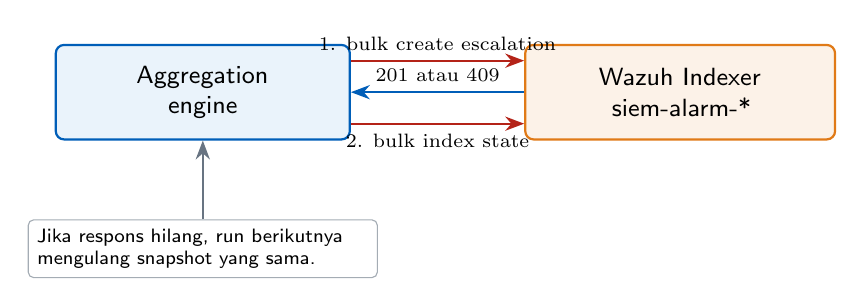
\begin{tikzpicture}[node distance=12mm and 22mm]
  \node[component] (engine) {Aggregation\\engine};
  \node[store,right=of engine] (indexer) {Wazuh Indexer\\\code{siem-alarm-*}};
  \node[note,below=10mm of engine] (retry) {Jika respons hilang, run berikutnya mengulang snapshot yang sama.};

  \draw[writeflow] ($(engine.east)+(0,4mm)$) -- node[above,font=\scriptsize]{1. bulk create escalation} ($(indexer.west)+(0,4mm)$);
  \draw[dataflow] ($(indexer.west)+(0,0mm)$) -- node[above,font=\scriptsize]{201 atau 409} ($(engine.east)+(0,0mm)$);
  \draw[writeflow] ($(engine.east)+(0,-4mm)$) -- node[below,font=\scriptsize]{2. bulk index state} ($(indexer.west)+(0,-4mm)$);
  \draw[flow] (retry) -- (engine);
\end{tikzpicture}
\caption{Urutan penulisan agar event tidak tertinggal di belakang state.}
\end{figure}

Bulk response diperiksa per item, bukan hanya status HTTP. Status 429, 502, 503,
dan 504 diulang dengan exponential backoff dan jitter. Hanya item yang gagal yang
diulang. Payload NDJSON dibekukan sehingga retry mengirim snapshot yang sama.

Batch dibatasi oleh jumlah action dan byte UTF-8. Dokumen tunggal yang lebih besar
dari batas menyebabkan run gagal sebelum write pertama. Ini mencegah keberhasilan
parsial yang sudah dapat diprediksi sejak awal.

\chapter{Checkpoint, Catch-Up, dan Late Alert}

Checkpoint menyimpan akhir bucket tertutup terakhir yang selesai, hash identitas
case, hash konfigurasi scoring, waktu update, dan metrik run. File ditulis ke temporary
file, di-flush, diubah permission menjadi 0600, lalu dipindahkan secara atomik.

Checkpoint bukan counter dan bukan sumber kebenaran alarm. Raw index tetap menjadi
sumber kebenaran. Fungsinya hanya mengatur recovery kalender agar outage tidak
menimbulkan query storm.

Pada bootstrap, engine hanya mengambil bucket finalized terbaru. Pada outage, jumlah
closed bucket yang diproses per run dibatasi, default dua. Bila source index untuk
bucket yang diperlukan tidak tersedia, run gagal dan checkpoint tidak maju. Operator
harus menyelidiki retensi atau menjalankan backfill terkontrol.

Manual backfill harus memakai waktu UTC yang aligned dengan boundary:

\begin{lstlisting}
--from 2026-04-21T02:00:00Z --to 2026-04-21T03:00:00Z
\end{lstlisting}

Backfill manual tidak memajukan checkpoint kalender. Timer dan service aktif harus
dihentikan agar tidak ada run dengan lock berbeda atau konfigurasi berbeda.

\begin{keypoint}
Late alert setelah finalisasi tidak otomatis memperbarui state. Ukur lag Filebeat
ke Indexer dan pertahankan p99 jauh di bawah delay finalisasi. Jika SLO tersebut
tidak dapat dicapai, naikkan delay atau jadwalkan prosedur reconciliation.
\end{keypoint}

\chapter{Fail-Closed dan Guardrail}

Engine memilih gagal tanpa menulis state parsial ketika menemukan keadaan yang
dapat membuat count salah. Contohnya:

\begin{itemize}
  \item timestamp, agent ID, rule ID, atau rule level wajib tidak valid;
  \item shard search gagal atau search timeout;
  \item tidak ada concrete daily index yang ter-resolve;
  \item total hit tidak eksak atau scroll berhenti sebelum seluruh hit diterima;
  \item alert per bucket melewati \code{max\_alerts\_per\_bucket};
  \item case unik melewati \code{max\_cases\_per\_bucket};
  \item response \code{\_mget} atau \code{\_bulk} malformed;
  \item asset inventory stale atau tidak valid;
  \item checkpoint rusak atau hash identitas berbeda.
\end{itemize}

Default cap 100.000 raw alert dan 20.000 case per bucket adalah ceiling keselamatan,
bukan kapasitas yang dijanjikan. Membagi bucket di tengah setelah cap tercapai akan
menghasilkan frequency salah, sehingga engine menolak pendekatan tersebut.
Initial scroll menggunakan \code{track\_total\_hits=true} karena Wazuh Indexer
4.14.7 menolak threshold numerik pada scroll context. Indexer karena itu menghitung
total hit eksak sebelum cap diperiksa. Cap tetap mencegah pagination, agregasi,
bulk, dan checkpoint untuk bucket yang terlalu besar, tetapi biaya exact-hit count
tetap harus diukur dalam load test.

Process lock berbasis \code{fcntl} mencegah dua instance Linux yang memakai lock file
sama berjalan bersamaan. Systemd \code{TimeoutStartSec=240s} membatasi eksekusi
\code{Type=oneshot} agar run tidak bertumpuk dengan jadwal berikutnya.

\chapter{Keamanan dan Least Privilege}

Koneksi ke Indexer wajib HTTPS dan verifikasi CA tidak dapat dimatikan melalui
config produksi. URL harus cocok dengan Subject Alternative Name sertifikat.
Runtime username \code{admin} serta password inline ditolak.

Role runtime yang disarankan:

\begin{table}[ht]
\centering
\caption{Hak minimum logis runtime.}
\begin{tabularx}{\textwidth}{l l X}
\toprule
\textbf{Scope} & \textbf{Pattern} & \textbf{Hak}\\
\midrule
Cluster & -- & \code{cluster\_composite\_ops\_ro}, clear-scroll, dan envelope bulk yang dibutuhkan.\\
Source & \code{wazuh-alerts-*} & Read-only.\\
Destination & \code{siem-alarm-*} & Read, index, dan create-index.\\
Tenant & -- & Tidak diperlukan.\\
Security/template/ISM & -- & Tidak diberikan kepada runtime.\\
\bottomrule
\end{tabularx}
\end{table}

Template dan ISM dipasang satu kali menggunakan administrator, kemudian
\code{install\_template=false}. Installer membuat service user tanpa login shell,
menolak managed symlink, membatasi filesystem melalui \code{ProtectSystem=strict},
menghapus Linux capabilities, mengaktifkan \code{NoNewPrivileges}, dan memberikan
write path hanya untuk log serta state.

Asset inventory root-owned lebih dipercaya daripada payload decoded. Label Wazuh
resmi hanya fallback. Pendekatan ini mengurangi risiko endpoint memalsukan nilai aset
melalui isi log yang dikirim.

\chapter{Performa dan Kapasitas}

Current bucket dihitung ulang setiap lima menit. Dengan laju relatif merata dan
12 run per jam, total scan current mendekati 5,5 kali jumlah alert satu bucket.
Finalisasi closed bucket menambah kira-kira satu kali, sehingga steady-state sekitar
6,5 kali jumlah alert per jam.

Jika satu bucket mengandung $A$ raw alert, estimasi dokumen yang dibaca per jam:

\[
  \text{scan per jam} \approx 6.5A
\]

Untuk $A=20.000$, sekitar 130.000 raw document dibaca sepanjang satu jam, meskipun
state akhir hanya mungkin beberapa ratus case. Penggunaan \code{\_mget} dan bulk
mengurangi round trip per case, tetapi tidak menghapus biaya scan snapshot.

Faktor kapasitas utama:

\begin{itemize}
  \item peak EPS dan burst di dalam bucket;
  \item jumlah rule/case unik;
  \item jumlah source IP, URL, user, dan file unik yang harus dicounter;
  \item heap, disk latency, dan shard pressure pada Indexer AIO;
  \item ukuran hasil JSON dan jumlah event escalation;
  \item waktu retry ketika Indexer menghasilkan 429.
\end{itemize}

Kriteria load test yang disarankan adalah traffic minimal dua kali peak aktual,
p95 run di bawah 60 detik, maksimum di bawah 240 detik, tanpa 429 atau failed shard,
dan tanpa menyentuh batas memory systemd.

\chapter{Dashboard dan Query Operasional}

Index pattern dashboard adalah \code{siem-alarm-*} dengan time field
\code{timestamp}. Karena state dan escalation berada pada index yang sama, semua
visualisasi wajib memfilter \code{document.type}.

Query state alarm terbaru:

\begin{lstlisting}
POST siem-alarm-*/_search
{
  "size": 50,
  "query": {
    "bool": {
      "filter": [
        {"term": {"document.type": "alarm_state"}},
        {"terms": {"risk.level": ["High", "Critical"]}}
      ]
    }
  },
  "sort": [{"alarm.last_seen": {"order": "desc"}}]
}
\end{lstlisting}

Query event yang dapat dikonsumsi aplikasi eksternal:

\begin{lstlisting}
POST siem-alarm-*/_search
{
  "size": 100,
  "query": {
    "bool": {
      "filter": [
        {"term": {"document.type": "alarm_escalation"}},
        {"range": {"event.created": {"gt": "<cursor-terakhir>"}}}
      ]
    }
  },
  "sort": [
    {"event.created": "asc"},
    {"escalation.id": "asc"}
  ]
}
\end{lstlisting}

Panel minimum mencakup total state per risk level, top agent, top rule, alarm High
dan Critical terbaru, top source IP, status open versus finalized, serta jumlah
escalation per waktu. Jangan menjumlahkan \code{alarm.event\_count} tanpa filter
state karena event escalation membawa snapshot alarm yang sama.

\chapter{Validasi Count terhadap Raw Evidence}

Validasi satu alarm dilakukan menggunakan identitas persisnya. Untuk contoh case
agent 002, rule 5503, bucket 02:00Z:

\begin{lstlisting}
POST wazuh-alerts-4.x-2026.04.21/_count
{
  "query": {
    "bool": {
      "filter": [
        {"term": {"agent.id": "002"}},
        {"term": {"rule.id": "5503"}},
        {"range": {
          "timestamp": {
            "gte": "2026-04-21T02:00:00Z",
            "lt":  "2026-04-21T03:00:00Z"
          }
        }}
      ]
    }
  }
}
\end{lstlisting}

Nilai \code{count} harus sama dengan tiga count pada \code{alarm\_state}. Untuk
mode target-aware, tambahkan filter destination sesuai case key. Untuk file-aware,
tambahkan path yang sama.

Validasi juga evidence:

\begin{itemize}
  \item cardinality source IP harus sama dengan \code{srcip\_unique\_count};
  \item terms aggregation source IP harus cocok dengan \code{top\_srcip};
  \item earliest dan latest timestamp harus cocok dengan first/last seen;
  \item source sample document ID harus benar-benar ada;
  \item asset source dan value harus sesuai inventory yang disetujui.
\end{itemize}

Perbedaan count tidak boleh langsung diperbaiki dengan mengedit state. Periksa
timezone index, filter rule, late alert, perubahan inventory/config, dan status
finalisasi; kemudian lakukan replay dari raw evidence bila diperlukan.

\chapter{Instalasi dan Urutan Go-Live}

Urutan implementasi yang aman:

\begin{enumerate}
  \item verifikasi versi paket dan semua service Wazuh aktif;
  \item verifikasi certificate chain, SAN, dan Filebeat output;
  \item jalankan seluruh unit test serta validator JSON;
  \item jalankan installer; pastikan timer tetap disabled;
  \item buat role dan user Indexer khusus;
  \item isi secret runtime dan inventory aset sebenarnya;
  \item pasang index template dan ISM policy menggunakan administrator;
  \item jalankan field audit pada traffic representatif;
  \item lakukan manual run, cek journal, lalu query state dan escalation;
  \item cross-check beberapa case terhadap raw alert;
  \item jalankan shadow/load test pada peak traffic;
  \item baru aktifkan timer dan monitor dua sampai tiga run pertama.
\end{enumerate}

Installer sengaja tidak mengaktifkan timer pada instalasi baru ataupun upgrade.
Jika timer sebelumnya enabled, installer menghentikan dan menonaktifkannya agar
operator melakukan validasi pasca-upgrade.

Index template harus ada sebelum write pertama agar daily index pertama menerima
mapping yang benar. ISM template hanya otomatis melekat pada index baru yang cocok;
index lama perlu diperiksa secara terpisah sebelum diberi policy.

\chapter{Monitoring Harian dan Troubleshooting}

Operator sebaiknya memantau:

\begin{itemize}
  \item hasil dan durasi unit systemd;
  \item 429, timeout, shard failure, cap exceeded, dan malformed response;
  \item waktu update checkpoint;
  \item jumlah state open/finalized;
  \item persentase \code{asset.source=default};
  \item p95/p99 lag raw alert ke Indexer;
  \item CPU, memory, heap, dan disk latency host AIO;
  \item adanya destination daily index dan status ISM.
\end{itemize}

\begin{longtable}{p{0.34\textwidth}p{0.58\textwidth}}
\toprule
\textbf{Gejala} & \textbf{Pemeriksaan awal}\\
\midrule
\endhead
Tidak ada alarm & Pastikan raw daily index ada, window benar, source filter tidak mengecualikan semuanya, dan refresh destination sudah terjadi.\\
Count lebih kecil & Periksa late alert, timestamp/index date, field wajib malformed, atau snapshot belum final.\\
Count lebih besar & Pastikan query pembanding menggunakan batas \code{gte}/\code{lt} dan filter case key yang sama.\\
Asset default & Lengkapi inventory, periksa agent ID/name, dan audit re-enrollment.\\
Service timeout & Ukur EPS/cardinality dan Indexer pressure; jangan langsung menaikkan cap.\\
Checkpoint mismatch & Ada perubahan identitas case; gunakan shadow prefix atau controlled migration.\\
Escalation tampak ganda & Filter berdasarkan \code{escalation.id}; create-only seharusnya menghasilkan satu ID per level.\\
\bottomrule
\end{longtable}

OnFailure saat ini mencatat pesan critical ke journald, tetapi tidak otomatis mengirim
email, webhook, atau tiket. Integrasi notifikasi eksternal perlu dibangun dari event
\code{alarm\_escalation} atau monitoring systemd.

\chapter{Batas Desain dan Tuning}

Default coarse adalah keputusan pengurangan noise, bukan kebenaran universal.
Satu rule failed login pada satu server dapat menyatukan banyak username dan source
IP. Ini berguna untuk melihat campaign terhadap host, tetapi tidak menghasilkan
satu alarm per akun. Mode \code{user\_aware} belum tersedia.

Demikian pula, sensor Suricata terpusat dapat menyatukan rule yang sama untuk banyak
destination. Gunakan override \code{target\_aware} atau
\code{target\_port\_aware}. Rule FIM yang memakai ID sama untuk banyak file umumnya
lebih mudah dianalisis dengan \code{file\_aware}.

Observed evidence dibatasi ketika dimaterialisasi, tetapi counter internal tetap
melihat semua nilai unik di snapshot. Cardinality ekstrem dapat menggunakan memory
besar sebelum dokumen diringkas. Cap alert, cap case, dan MemoryMax menjadi lapisan
pertahanan; hasil load test menentukan apakah rule noisy perlu dikecualikan.

Skor rata-rata tiga komponen tidak memasukkan business impact selain asset value,
control effectiveness, exposure, threat intelligence, confidence, atau analyst
feedback. Tuning skor harus dimulai dari kebijakan tertulis dan contoh kasus, lalu
diuji menggunakan shadow destination. Jangan mengubah threshold langsung pada
index produksi tanpa rencana backfill dan interpretasi dashboard baru.

\chapter{Checklist Penerimaan Produksi}

Gunakan daftar berikut sebagai keputusan go/no-go:

\begin{itemize}[label=$\square$]
  \item Paket Wazuh dan Filebeat sama dengan baseline yang direview.
  \item TLS berhasil tanpa insecure mode; URL cocok dengan SAN.
  \item Runtime bukan admin dan role lulus uji read/mget/scroll/bulk/create-index.
  \item Template dan ISM terpasang sebelum destination index dibuat.
  \item Inventory seluruh agent penting lengkap; asset default tidak boleh muncul tanpa rencana.
  \item Field audit mencakup custom decoder dan rule produksi.
  \item \code{bucket\_minutes=60} dan index date terbukti mengikuti UTC.
  \item Minimal satu state dan satu escalation aktual sudah diverifikasi.
  \item Tiga count state sama dan cocok dengan query raw evidence.
  \item Current state berkembang dan closed bucket menjadi finalized.
  \item Late-alert SLO berada di bawah finalization delay.
  \item Failure injection membuktikan retry tidak menduplikasi event.
  \item Load test dua kali peak memenuhi p95 dan TimeoutStartSec.
  \item Checkpoint owner/mode benar dan bergerak hanya setelah run sukses.
  \item Dashboard memfilter document type dengan benar.
  \item Monitoring service failure dan prosedur backfill sudah dimiliki operator.
  \item Rollback window, backup, dan PIC keputusan sudah ditetapkan.
\end{itemize}

Go-live dinyatakan berhasil setelah beberapa bucket aktual melewati lifecycle open,
escalation, dan finalized tanpa count drift, late-alert loss, atau degradasi Indexer.

\chapter{Kesimpulan}

Sistem ini membentuk lapisan agregasi yang dapat dijelaskan: satu identitas case,
satu state deterministik, bukti observed yang diringkas, dan event escalation yang
immutable per level. Raw Wazuh tidak disentuh, sehingga investigasi tetap dapat
kembali ke dokumen asal.

Untuk baseline satu jam, rumus dan implementasi konsisten. Source IP berbeda
diagregasikan sebagai counter dan sampel, bukan di-replace. Progressive snapshot
menghindari double count, sedangkan two-phase bulk, deterministic ID, lock, dan
checkpoint menyediakan recovery yang aman.

Nilai praktis sistem bergantung pada tiga disiplin: memilih mode deduplikasi per
rule, memelihara inventory aset, dan mengukur lag serta kapasitas pada traffic nyata.
Tanpa ketiganya, agregasi tetap berjalan tetapi dapat terlalu kasar, salah prioritas,
atau terlambat memfinalisasi bukti.

Keputusan yang direkomendasikan adalah menjalankan shadow deployment terlebih dahulu,
mempertahankan bucket 60 menit, memperbaiki contoh dokumentasi agar menjadi golden
test, dan memberikan status production hanya setelah checklist penerimaan terpenuhi.

\appendix

\chapter{Ringkasan Konfigurasi Baseline}

\begin{lstlisting}
{
  "opensearch_url": "https://127.0.0.1:9200",
  "username": "siem_alarm_service",
  "password_env": "WAZUH_PASS",
  "verify_ssl": true,
  "ca_cert": "/opt/wazuh-risk-scoring/root-ca.pem",
  "source_index": "wazuh-alerts-4.x-{date}",
  "destination_index_prefix": "siem-alarm",
  "deduplication_mode": "coarse",
  "bucket_minutes": 60,
  "process_current_bucket_only": true,
  "lookback_overlap_minutes": 7,
  "escalation_log_enabled": true,
  "escalation_log_levels": ["Medium", "High", "Critical"],
  "threat_level_strategy": "max",
  "max_alerts_per_bucket": 100000,
  "max_cases_per_bucket": 20000,
  "page_size": 1000,
  "mget_batch_size": 1000,
  "bulk_max_actions": 1000,
  "bulk_max_bytes": 5242880,
  "max_catchup_buckets_per_run": 2,
  "install_template": false
}
\end{lstlisting}

Key lain seperti timeout, retry, evidence limits, exclusions, log path, lock path,
assets path, dan checkpoint path harus dipertahankan dari config lengkap. Cuplikan
ini adalah baseline penjelasan, bukan pengganti file proyek.

\chapter{Matriks Field Output}

\begin{longtable}{>{\ttfamily\raggedright\arraybackslash}p{0.36\textwidth}p{0.56\textwidth}}
\toprule
\normalfont\textbf{Field} & \textbf{Makna}\\
\midrule
\endhead
document.type & Memisahkan alarm state dan escalation event.\\
alarm.id & SHA-256 case key dan document ID state.\\
alarm.case\_key & Identitas kasus yang dapat diaudit.\\
alarm.status & Lifecycle bucket, bukan workflow analis.\\
alarm.first\_seen / last\_seen & Batas timestamp event dalam snapshot.\\
alarm.event\_count & Jumlah raw document case.\\
rule.level & Level terpilih menurut strategy.\\
rule.level\_counts & Distribusi level pada snapshot.\\
source\_observed.top\_srcip & Source IP paling sering beserta count terbatas.\\
target\_observed.* & Destination, port, dan protocol yang diamati.\\
entity\_observed.* & User, URL, user agent, file, hash, CVE, dan SCA.\\
asset.* & Nilai, kategori, owner, environment, dan sumber metadata aset.\\
risk.score / level & Skor rata-rata dan kategori hasil.\\
risk.previous\_level & Level state sebelum update saat ini.\\
risk.level\_history & Riwayat kenaikan level di dalam bucket.\\
source.raw\_alert\_count & Counter raw yang harus sama dengan event count.\\
source.sample\_document\_id & Pointer ke raw sample paling awal secara deterministik.\\
soc.recommended\_action / sla & Saran tindakan berbasis risk level.\\
escalation.state\_alarm\_id & Relasi event immutable ke state.\\
event.created & Waktu event escalation dimaterialisasi.\\
\bottomrule
\end{longtable}

\chapter{Glosarium}

\begin{description}[style=nextline,leftmargin=30mm]
  \item[AIO] All-in-one; manager, indexer, dan dashboard berada pada satu host.
  \item[Bucket] Rentang waktu tetap untuk membentuk identitas dan frequency count.
  \item[Case key] String deterministik yang mendefinisikan satu alarm agregat.
  \item[Checkpoint] Penanda recovery bucket tertutup yang sudah selesai.
  \item[Current bucket] Bucket waktu yang masih berjalan dan dihitung ulang.
  \item[Closed bucket] Bucket yang boundary akhirnya telah lewat.
  \item[Finalized] Snapshot closed bucket telah berhasil ditulis.
  \item[Evidence] Nilai pendukung seperti IP, user, URL, port, file, atau CVE.
  \item[Idempotent] Operasi aman diulang tanpa membuat hasil logis ganda.
  \item[Late alert] Alert yang baru terlihat di Indexer setelah finalisasi bucket.
  \item[Raw alert] Dokumen deteksi asli pada \code{wazuh-alerts-*}.
  \item[Shadow run] Menjalankan engine ke destination terpisah tanpa menjadi sumber operasi utama.
  \item[State] Representasi terbaru satu kasus dalam bucket.
  \item[Escalation] Event immutable ketika level eligible pertama muncul atau meningkat.
\end{description}

\chapter{Referensi Teknis}

\begin{thebibliography}{9}
\bibitem{wazuhrelease}
Wazuh, \emph{Wazuh 4.14.7 Release Notes}.\\
\url{https://documentation.wazuh.com/current/release-notes/release-4-14-7.html}

\bibitem{wazuhindices}
Wazuh, \emph{Wazuh Indexer Indices}.\\
\url{https://documentation.wazuh.com/current/user-manual/wazuh-indexer/wazuh-indexer-indices.html}

\bibitem{wazuhrules}
Wazuh, \emph{Rules Classification}.\\
\url{https://documentation.wazuh.com/current/user-manual/ruleset/rules/rules-classification.html}

\bibitem{wazuhsshrules}
Wazuh, \emph{Wazuh 4.14.7 default SSHD rules, 0095-sshd\_rules.xml}.\\
\url{https://github.com/wazuh/wazuh/blob/v4.14.7/ruleset/rules/0095-sshd_rules.xml}

\bibitem{wazuhlabels}
Wazuh, \emph{Agent Labels}.\\
\url{https://documentation.wazuh.com/current/user-manual/agent/agent-management/labels.html}

\bibitem{osbulk}
OpenSearch, \emph{Bulk API}.\\
\url{https://docs.opensearch.org/latest/api-reference/document-apis/bulk/}

\bibitem{osmget}
OpenSearch, \emph{Multi-get Documents API}.\\
\url{https://docs.opensearch.org/latest/api-reference/document-apis/multi-get/}

\bibitem{osism}
OpenSearch, \emph{Index State Management Policies}.\\
\url{https://docs.opensearch.org/latest/im-plugin/ism/policies/}

\bibitem{projectreadme}
Proyek SIEM Alarm, \projectfile{README.md},
\projectfile{final\_checklist\_siem\_alarm\_wazuh\_4\_14\_7.md}, dan source code
yang berada pada repository yang sama dengan dokumen ini.
\end{thebibliography}

\vfill
\begin{center}
\color{LineGray}\small
Akhir dokumen --- Logika Agregasi SIEM Alarm untuk Wazuh 4.14.7 AIO
\end{center}

\end{document}
